\section{Implementation}
\label{sec:implementation}

In this section, we detail our implementation on Arduino \cite{Arduino} platform. The whole system is comprised of a glass module, numbers of clients, and a gateway, as shown in the architecture figure (Fig.\,\ref{fig:sysarch}) in last section. We will start from the clients, whose primary tasks are to interface between the Glass and the devices that are attached to it. Then we move on to the implementation of the Glass, who manges users' gesture recognition and communication with clients. The functionality in gateway so far is only minimum to communicate with clients, since it's not the primary focus of this project.

\subsection{Clients}
The clients are comprised of a main Arduino board, an IR receiver, an XBee radio, and various actuators. We used Arduino Uno, which has an ATmega328 microcontroller and suffice our purpose in this project. We use off-the-shell IR receivers ({\color{red} confirm it is PNA4602}), which outputs 0V (low) on detection of 38 KHz carrier or 5V (high) otherwise. The XBee radio, accompanied with an XBee modems, takes charge of the communication with the Glass. LEDs are added as an indicator of the state of clients and visual feedback for users. Additional components are subject to the device being attached to. In our current system, we have a relay ({\color{red} need to know relay model}) which can control the AC power plug, and we have a USB connected computer to control video playing. The prototype is shown in Fig.\,\ref{fig:client}.

{\color{red} add clients photos here}
\begin{figure}
  \centering
%  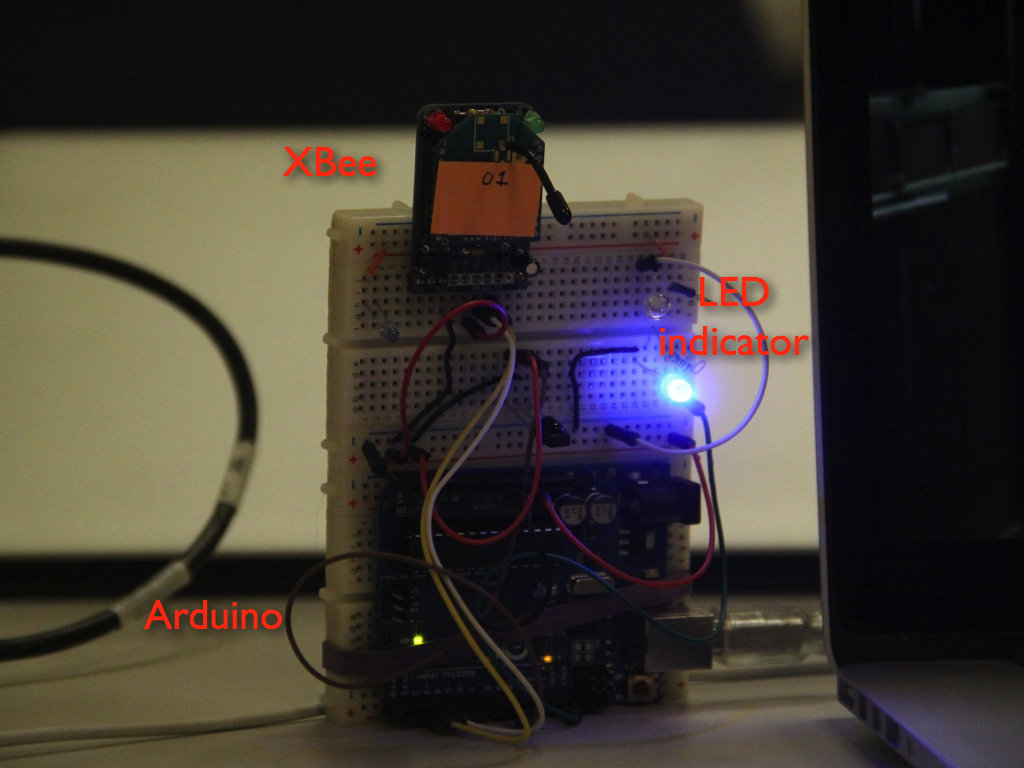
\includegraphics[width=\linewidth]{../figs/client.png}
  \caption{Prototype of the clients}
  \label{fig:client}
\end{figure}

The main function of the client is to respond IR signal, and communicate with the Glass to receive corresponding commands. Normally, the client lives in {\it IDLE} mode. When they receive IR signals, indicating the user is expressing interest in interacting with it, the client responds with an XBee acknowledgement and goes into {\it PENDING} state. In this case, since the client doesn't know how many other clients have also responded to the glass, it will wait until a connection signal. If there are multiple clients waiting to be verified by the Glass, the coordination is done at the Glass through sending the right verifying message. To provide visual feedback to the user, the active client that is being verified will blink faster. When it receives the connecting message, it goes to {\it CONNECTED} state and is now ready to take commands. To summarize the clients' behavior, we have a state machine in Fig.\,\ref{fig:clientFSM} for illustration.

\begin{figure}
  \centering
  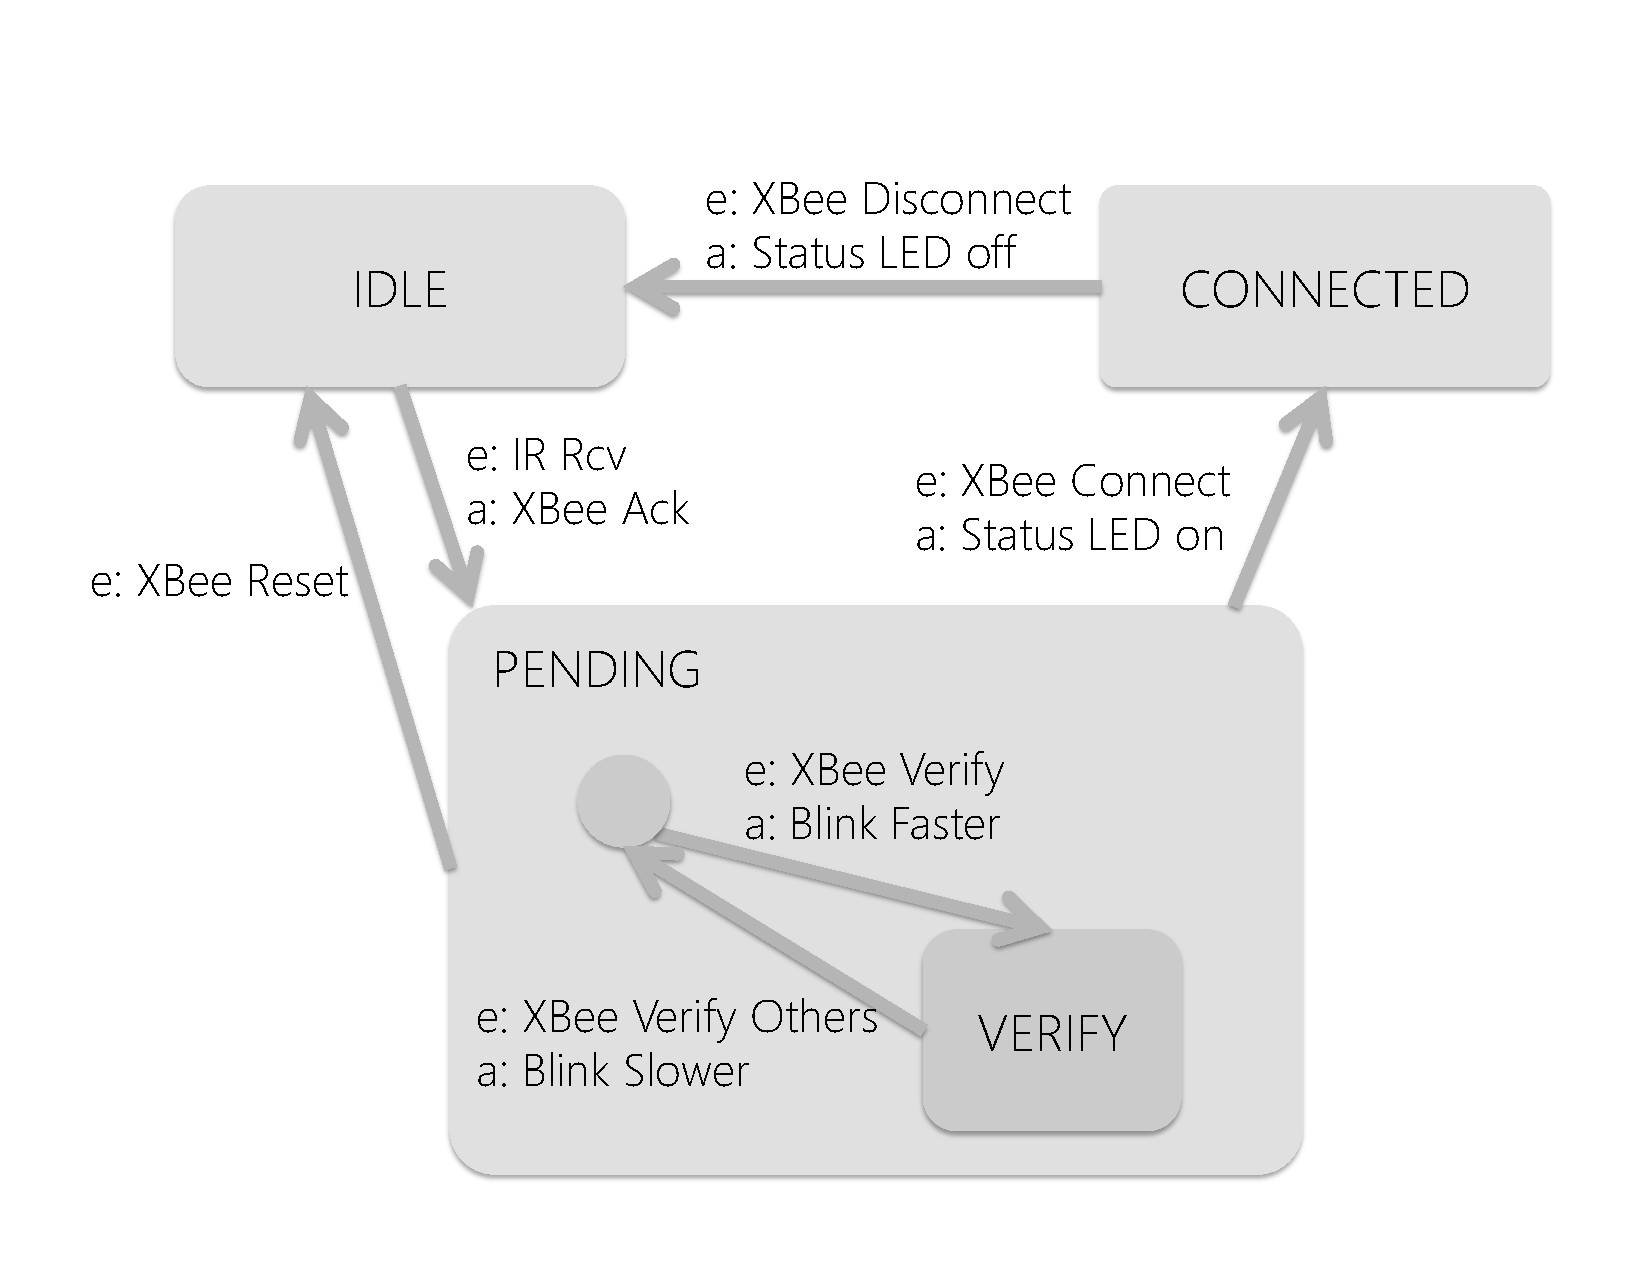
\includegraphics[width=\linewidth]{../figs/clientFSM.pdf}
  \caption{FSM model for client. For each transition, ``e'' stands for event, and ``a'' stands for action}
  \label{fig:clientFSM}
\end{figure}

Within {\it CONNECTED} state, the clients will react differently according to the device it is connected to. In our prototype, we have two different types of devices. The first is a relay, which can control the whole AC power supply. The interface to relay is simply an digital pin. We only need to set it to {\it LOW} or {\it HIGH}. Such command is transmitted remotely from the Glass through XBee using encoded packet. The second tyep is a computer that is used to play video. To send command to the computer, we have a USB adaptor and a python script taking charge of the translation. We use {\it pyserial} and {\it appscript} in the software. And this enables controlling the play and pause of an video, and system-wide volume control.

\subsection{Glass}
\label{sec:glass}

The Glass is complicated in two folds. First, we move the complexity of coordinating all clients to the Glass. Second, we have to handle user gesture on Glass. From an engineer perspective, we separate the gesture detection and XBee transmission into two customized library files in Arduino. And only interesting information is exposed to the main program. We use the same Arduino Uno and XBee module as the client. In addition, we have a membrane potentiometer (100 mm long) as the slider to take user's input, and the most important IR emitter to broadcast IR signals. After we've put the components onto the Glass, we have the prototype shown in Fig.\,\ref{fig:glass}.

{\color{red} add glass photos here}
\begin{figure}
  \centering
  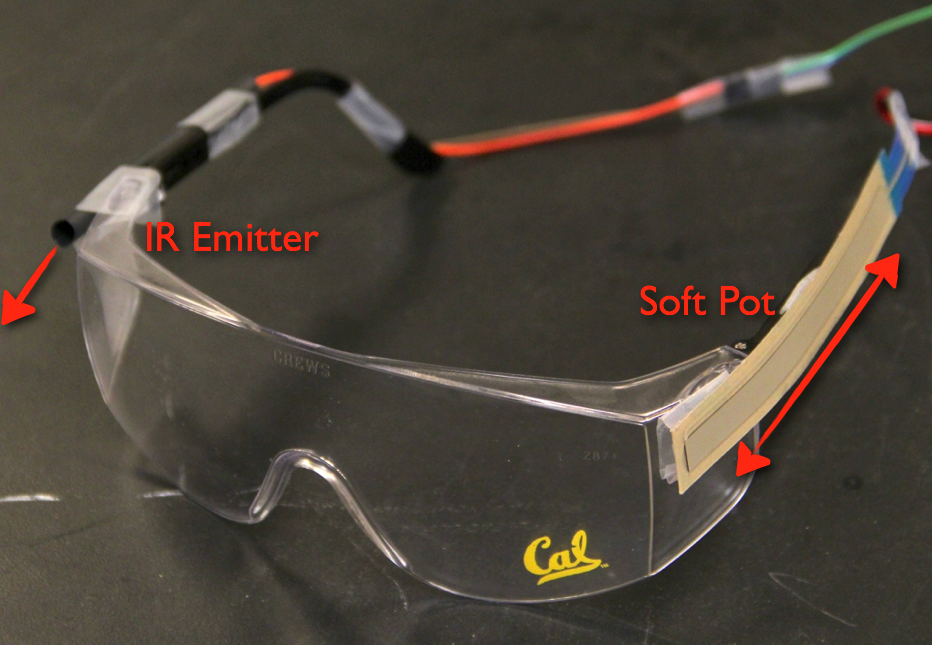
\includegraphics[width=0.85\linewidth]{../figs/glass.png}
  \caption{Prototype of the Glass}
  \label{fig:glass}
\end{figure}


The whole work flow on the Glass is as follows. When the user hasn't shown any interest for interaction, the system stays in {\it IDLE} state. When ``tapping'' is detected, the Glass will broadcast IR signals to inform the devices which are in front of the user. Since we have the tube around the IR transmitter, the resulting signal coverage is a pretty straight line. After the Glass has sent out IR message, at this time, it doesn't know how many devices might respond. In this case, the Glass would wait for a specific period of time, and count the number of acknowledgement messages sent by clients. To ensure responsiveness to end user, we set the timer in {\it WAIT} state to be 1 second. When the timer expires, Glass will go to {\it IDLE} if no client has responded, or {\it CONFIRM} if it receives just one message. However, the complicated case is when there are multiple clients that have received the IR signal (because they are near to each other) and responded. Though we expect this scenario rarely happens, there is still chance when the physical devices are put together and it is necessary to differentiate them. In this case, the system goes to {\it VERIFY} state, and sends out corresponding verifying message based on user's gesture. We adopt the slider on glass to change active selection. Once the user confirmed the selection, it goes to {\it CONNECTED} state and now the Glass is ready to send out commands. We have the FSM in Fig.\,\ref{fig:glassFSM}.

We've configured the XBee modules such that the Glass can talk in both direction with all clients, while clients cannot talk with each other. In this way, the Glass would serve as master of this personal area network (PAN), whose ID is 4321 in our scenario. 

\begin{figure}
  \centering
  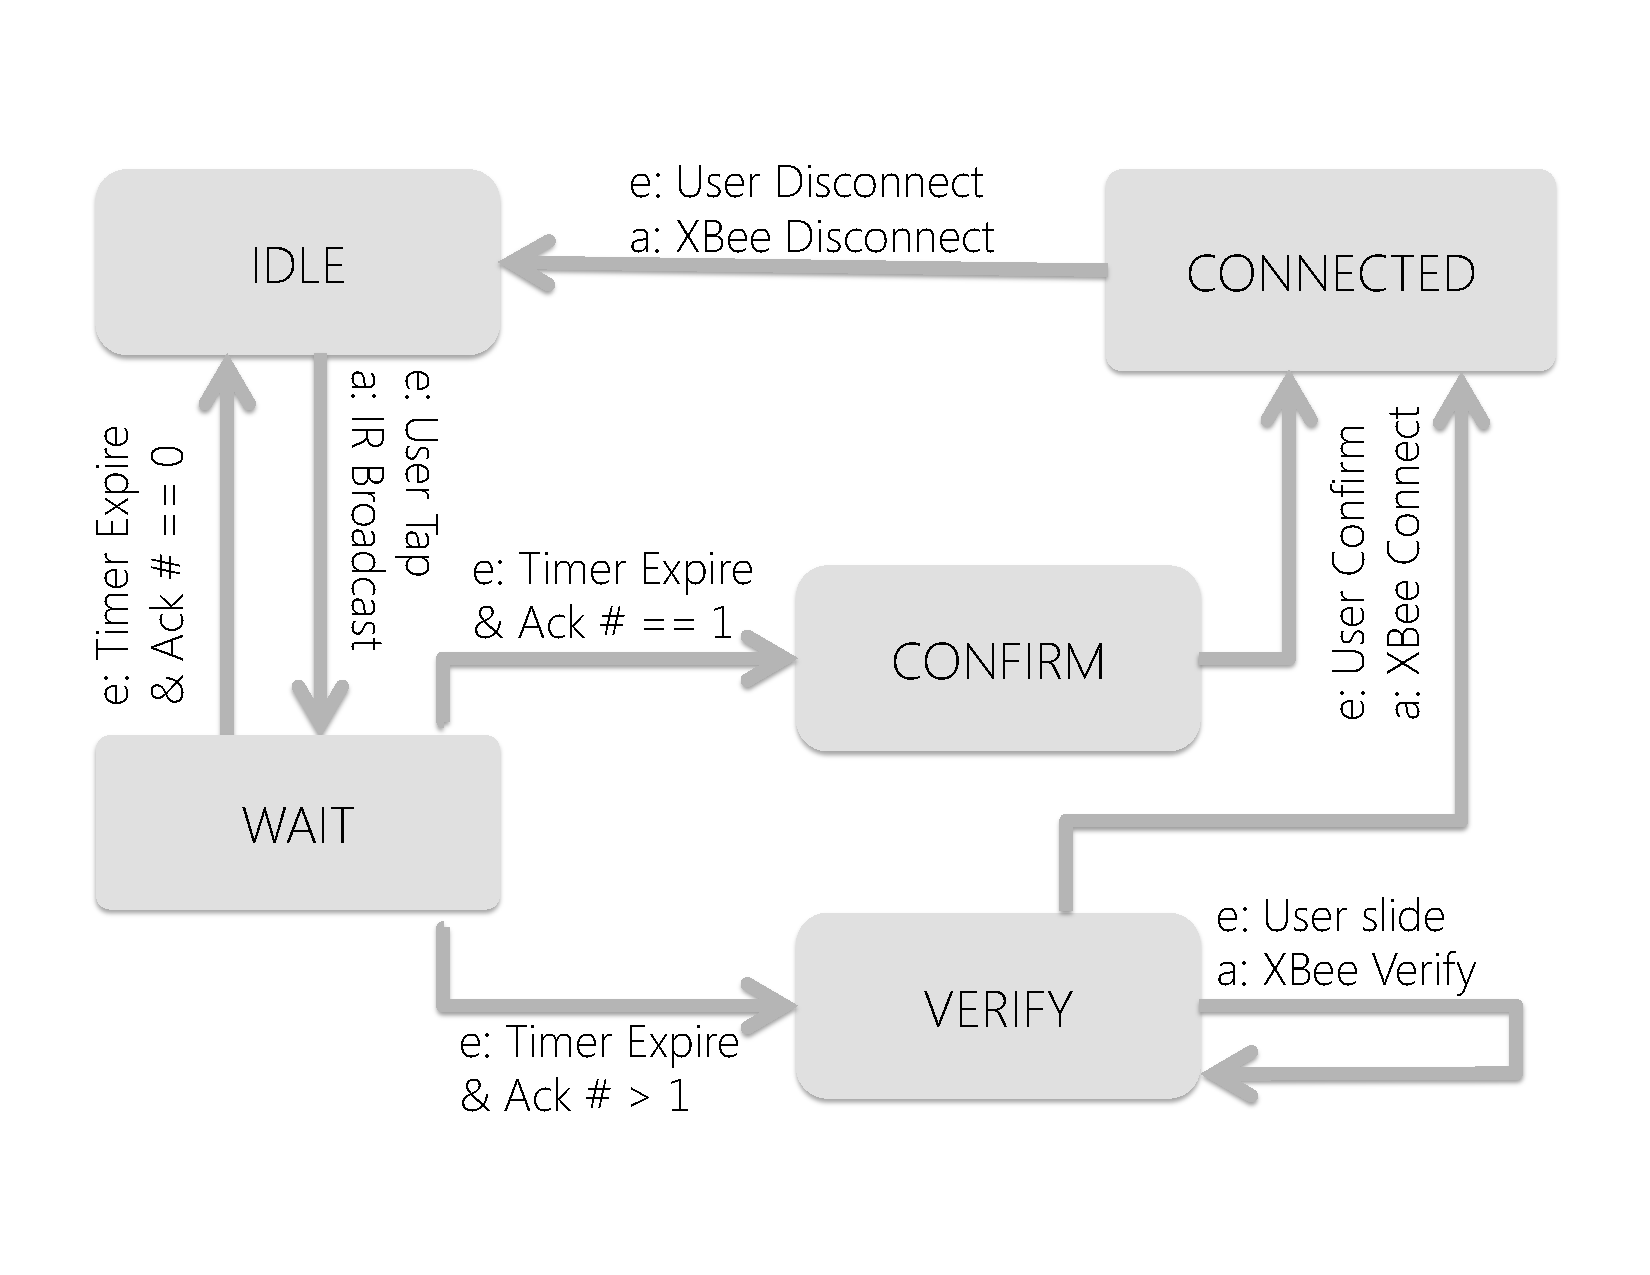
\includegraphics[width=\linewidth]{../figs/glassFSM.pdf}
  \caption{FSM model for Glass. For each transition, ``e'' stands for event, and ``a'' stands for action}
  \label{fig:glassFSM}
\end{figure}

\subsection{Gateway}
\label{sec:gateway}

The gateway provides access to this PAN for computers, and presumably this can be further open to the Internet. Since there have already been many products \cite{NinjaBlocks, Lockitron} that essentially function in this way, we do not spend much time on this aspect in our project. 

For completeness, we wrote a python script that controls a USB XBee adaptor. And this XBee module has the same configuration as the Glass, so it serves as the master of the network. This enables the remote control of the clients.


%%% Local Variables: 
%%% mode: latex
%%% TeX-master: "main"
%%% End: 
